% !TEX encoding = UTF-8
% !TEX TS-program = pdflatex
% !TEX root = ../tesi.tex

%**************************************************************
\chapter{Introduzione}
\label{cap:introduzione}
%**************************************************************


% \noindent Esempio di utilizzo di un termine nel glossario \\
\gls{apig}. \\
\gls{umlg}
\gls{VoiPg}
% \noindent Esempio di citazione in linea \\
% \cite{site:agile-manifesto}. \\

% \noindent Esempio di citazione nel pie' di pagina \\
% citazione\footcite{womak:lean-thinking} \\
\intro{In questo capitolo viene descitta l'azienda dove in cui è stato svolto lo stage e viene spiegato  il progetto di stage.}\\
%**************************************************************
\section{SyncLab }
SyncLab è una Innovative Company collocata in tutta italia, è nata nel 2002 con sede principale a Napoli ed è cresciuta velocemente. Attualmente, SyncLab ha 6 sedi in tutta italia, più di 300 dipendenti e più di 150 clienti diretti e finali.\\
SyncLab propone servizi innovativi che aiutano i clienti nella realizzazione, progettazione e manutenzioni di soluzioni IT.
L'azienda ha collobarobato con vari compagnie tra questi i più importanti sono: Tim, Trenitalia, HM, Grimaldi Lines, notartel, sky, eni, enel, vodafone, RayWay, Poste Italiane, Intesa Sanpaolo, Ministero dell'economia delle finanze, fastweb e UniCredit.
\begin{figure}[H]
    \centering
    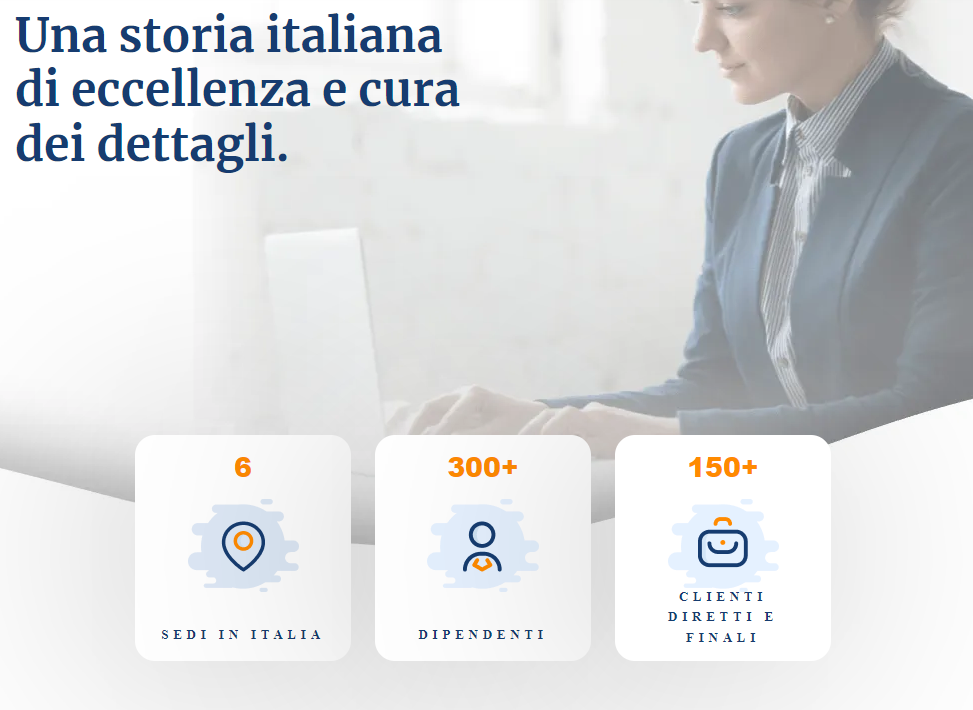
\includegraphics[scale=0.50]{azienda.png}
    \caption{Punti di forza di SyncLab}
\end{figure}
\subsection{Prodotti}
Come accenato, SyncLab opera nel settore IT e i suoi prodotti nascono dalle competenze acquisite e maturate durante le loro 20 anni di collaborazioni. I prodotti coprono vari ambiti come quelli delle telecomunicazioni, utilities, finanza e salute.
\begin{figure}[H]
    \centering
    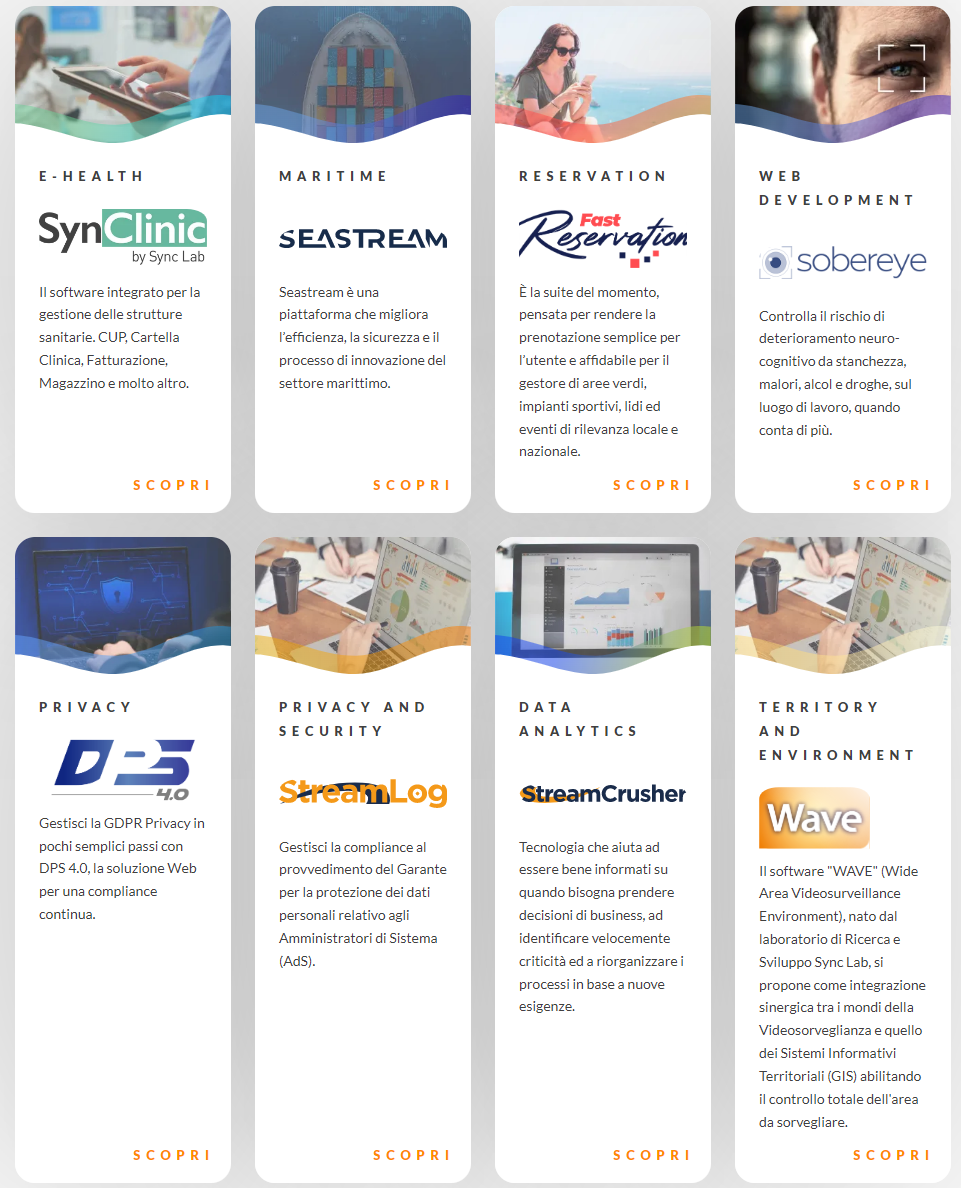
\includegraphics[width=1.0\textwidth]{prodotti.png}
    \caption{I vari prodotti di SyncLab}
\end{figure}
\begin{itemize}
    \item \textbf{SynClinic:} software integrato per la gestione delle strutture sanitarie, come il sistema di cartella clinica digitale, il servizio di fatturazione, la gestione informatizzata dei farmaci, i strumenti nativi di gestione amministrativa e tanto altro.
    \item \textbf{SEASTREAM:} una piattaforma nata per migliorare e potenziare le attività di business nel settore armatoriali e di altri operatori del mercato marittimo
    \item \textbf{FastReservation:} applicazione realizzato per rendere il sistema di prenotazione più facile e affidabile per gli utenti.
    \item \textbf{Sobereye:} soluzione per la sicurezza proattiva per la prevenzione degli incidenti nei settori di trasporti, estrazione, costruzioni e industrale.
    \item \textbf{DPS 4.0:} applicativo che permette di gestire la GDPR Privacy Policy. L'applicativo, tramite una guida semplice sviluppata dagli ingegneri esperti nell'ambito dei user experience, offre la possibilità di modificare e aggiornare i documenti sulla privacy con il minimo sforzo.
    \item \textbf{StreamLog:} soluzione per la protezione dei dati personali relativo agli Amministratori di Sistema, dà possibilità di effettuare il controllo degli accessi degli utenti ai sistemi in modo semplice ed efficace.
    \item \textbf{StreamCrusher:} tecnologia che serve per aiutare a prendere decisioni di business, indentificando velocemente i punti critici e riformando i processi in base alle nuove esigenze.
    \item \textbf{Wave:} software nato per i sistemi di vidersorverglianza, con l'obiettivo di avere una maggiore copertura territoriale col minor numero di telecamere installate e possibilmente utilizzare il minor numero possibile di risorse.
\end{itemize}
\begin{figure}[H]
    \centering
    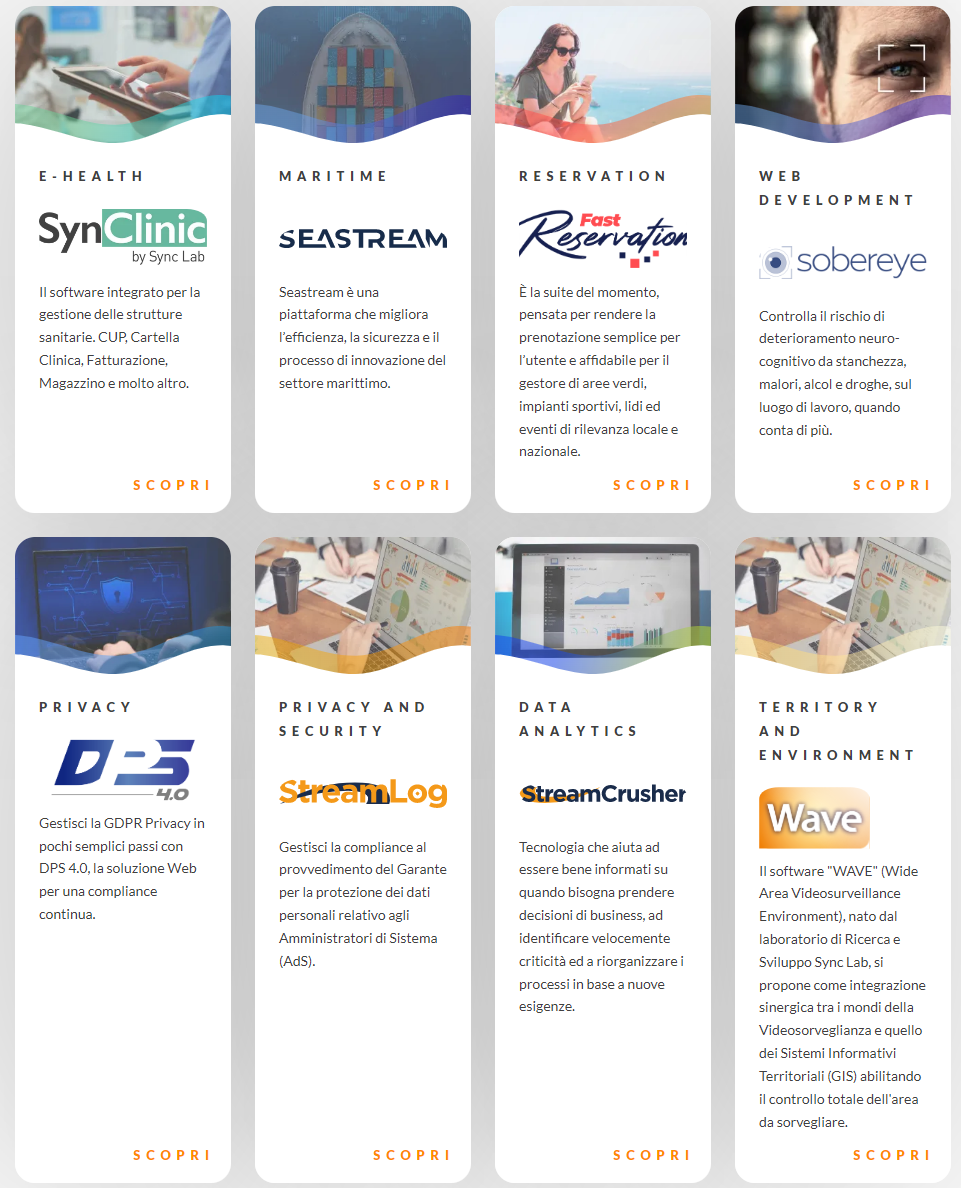
\includegraphics[width=1.0\textwidth]{prodotti.png}
    \caption{I vari prodotti di SyncLab}
\end{figure}

\subsection{Introduzione al progetto}
Lo scopo dello stage quello di realizzare una web-app per la gestione delle ordinazione dei piatti di un ristorante sushi "all you can eat", con tale formula i ristoranti offrono la possibilità di ordinare senza limiti ad un prezzo fisso, oltre a questo il menù contiene una centinaia di piatti diversi. Quindi i consumi dei clienti in questi locali è maggiore rispetto ai ristoranti tradizionali, perché con la formula "all-you-can-eat" spesso i clienti mangiano oltre il loro livello di sazietà, di seguito comporterà un elevato numero di ordinazioni da gestire creando così il problema di capire poi chi ha ordinato il specifico piatto nel momento della consegna.

\section{La soluzione individuata}
SyncLab ha deciso di risolvere questo problema tramite una web-app, che è composta da due parti la parte front-end e la parte back-end. La parte di back-end deve essere implementata tramite java utilizzando il framework spring e ha il ruolo pricipale di un web server, che deve comunicare con il data-base, dove vengono salvati tutte le informazioni dei piatti e tutti gli ordini effettuati dai clienti.
La parte di front-end è invece realizzato in Javascript, utilizzando il framework Angular. La comunicazione tra le due parti della web-app avviene tramite le chiamate REST fornite dal back-end.
Si è deciso di realizzare una web-app perché non c'è la necessità di scaricare ed installare applicativo, così riduce il tempo delle ordinazioni dei clienti. 

\begin{figure}[H]
    \centering
    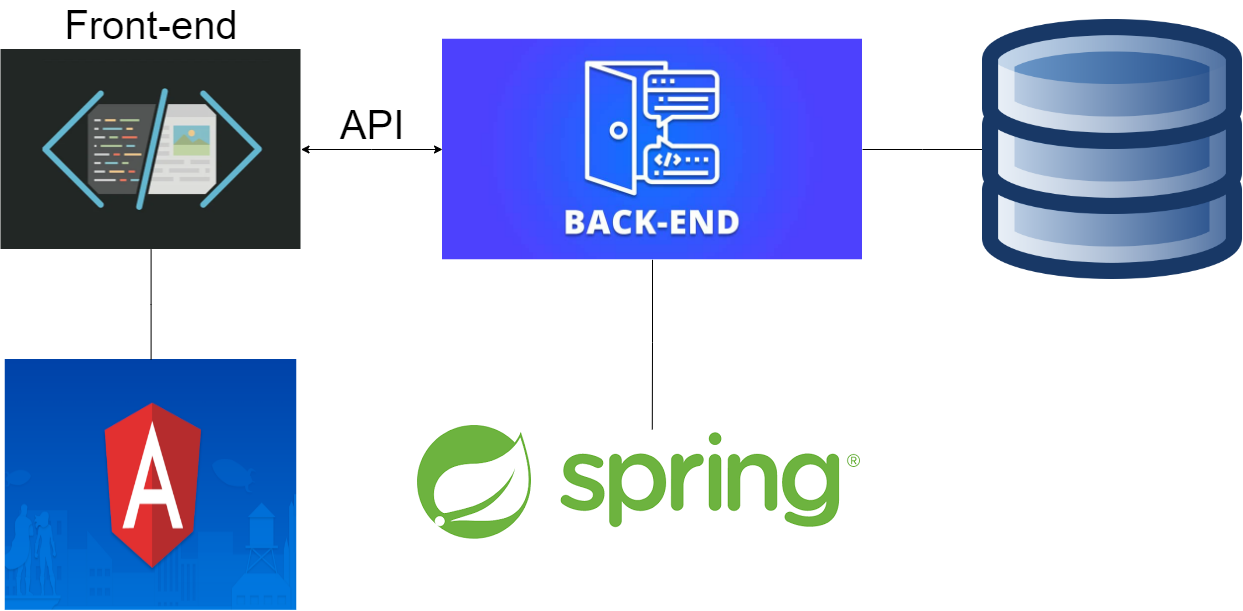
\includegraphics[scale=0.27]{diagramma.png}
    \caption{Diagramma dei componenti per la web-app}
\end{figure}
%**************************************************************


%**************************************************************
\section{Organizzazione del testo}

\begin{description}
    \item[{\hyperref[cap:il progetto di stage]{Il secondo capitolo}}] descrive in dettaglio il progetto di stage, il problema individuato e una sua soluzione.
    
    \item[{\hyperref[cap:analisi dei requisiti]{Il terzo capitolo}}] descrive l'analisi dei requisiti della web-app, vengono discussi tutti i casi d'uso e i requisiti da rispettare.
    
    \item[{\hyperref[cap:progettazione e codifica]{Il quarto capitolo}}] approfondisce la progettazione e codifica, elencando i vari componenti e descrivendo le loro funzionalità.
    
    % \item[{\hyperref[cap:progettazione-codifica]{Il quinto capitolo}}] approfondisce ...
    
    \item[{\hyperref[cap:verifica]{Il quinto capitolo}}] approfondisce la fase di verifica e validazione della web-app.
    
    \item[{\hyperref[cap:conclusioni]{Nel sesto capitolo}}] vengono trattate le conclusioni dell'intero progetto, parlando del prodotto finale e le competenze acquisite durante lo stage.
\end{description}
Riguardo la stesura del testo, relativamente al documento sono state adottate le seguenti convenzioni tipografiche:
\begin{itemize}
	\item gli acronimi, le abbreviazioni e i termini ambigui o di uso non comune menzionati vengono definiti nel glossario, situato alla fine del presente documento;
	\item per la prima occorrenza dei termini riportati nel glossario viene utilizzata la seguente nomenclatura: \emph{parola}\glsfirstoccur;
	\item i termini in lingua straniera o facenti parti del gergo tecnico sono evidenziati con il carattere \emph{corsivo}.
\end{itemize}